%\documentclass[../document.tex]{subfiles}
%\begin{document}

\chapter{Classificazione Multiclasse}
Di seguito una presentazione dei due schemi di aggregazione per classificatori binari che consentono di ottenere classificatori $k$-ari, nonché il criterio di unificazione fra essi --- oggetto di questo elaborato.

\section{Metodo one-vs-all}
Sia $T$ un \textit{dataset} di $k$ classi di punti ($k = |C|$). Si supponga per semplicità di notazione che le etichette di classe siano $C = \left\{ 1, 2, \; ... \;, k \right\}$. Questo metodo consente di costruire un classificatore $k$-ario a partire da $k$ classificatori binari (e.g. \textit{SVM}); ciò è realizzato --- come ben espresso dal nome alternativo \textit{one-vs-rest} --- considerando di volta in volta la $i$-esima classe ($i \in C$) ``contro'' il resto dei punti.
Più formalmente, per il classificatore $i$-esimo, la classe dei positivi e quella dei negativi sono così definite:
\begin{equation}
	T_{i_+} = \left\{ \boldsymbol{x}_+ \in \mathbb{R}^d \;|\; (\boldsymbol{x}_+, i) \in T \right\}	
\end{equation}
\begin{equation}
	T_{i_-} = \left\{ \boldsymbol{x}_- \in \mathbb{R}^d \;|\; (\boldsymbol{x}_-, j) \in T ;\; j \neq i \right\}		
\vspace{2mm}
\end{equation}

Il classificatore $i$-esimo è addestrato dunque su di esse.
I positivi $T_{i_+}$ sono tutti i punti di classe $i$; i negativi $T_{i_-}$ sono tutti i punti di classe diversa da $i$.
Una descrizione grafica di questa selezione è data in Figura A.

\begin{figure}[H]
 	\centering	
	
	\fboxsep=0mm%padding thickness
	\fboxrule=1mm%border thickness

	\fcolorbox{border_color}{white} {
		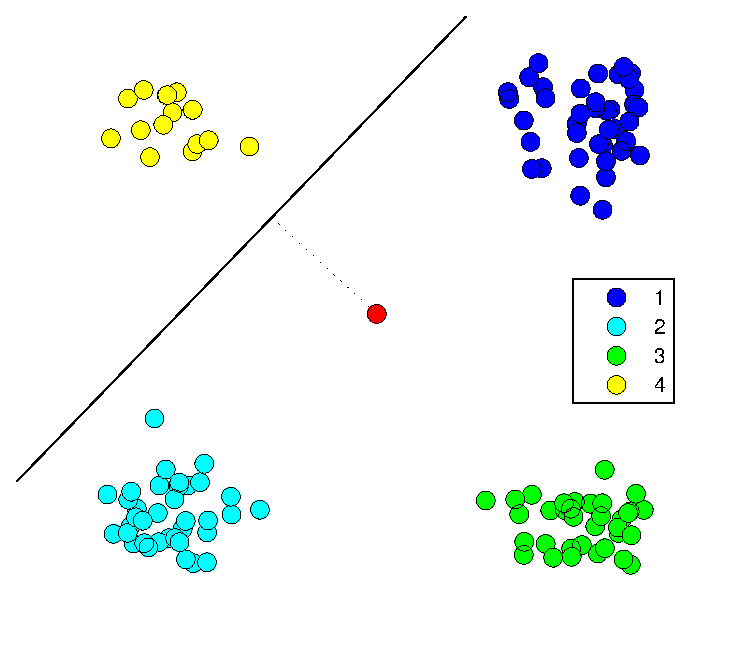
\includegraphics[scale=1]{img/1vsall.eps}		
		%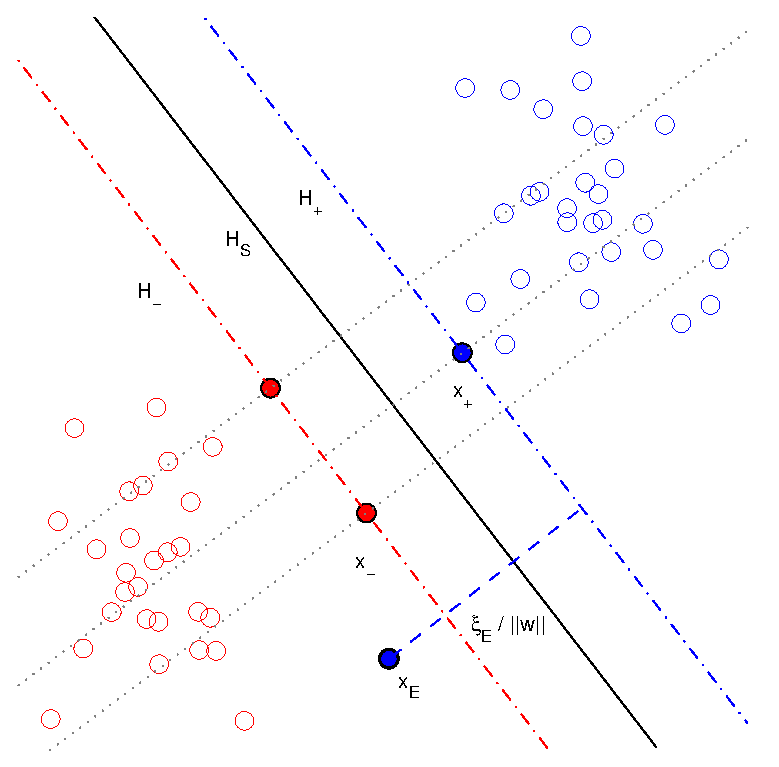
\includegraphics[scale=1]{../img/FiguraE_soft.eps}
	}	
	\caption{Esempio di iperpiano per classe 4 vs rest in $\mathbb{R}^2$. (con kernel lineare) L'elemento in rosso rappresenta un vettore di test}
	%Si noti che la sua distanza da $H_-$ è $\xi_E / ||w||$}
\end{figure}

\paragraph{}
Completata la fase di training, resta da definire in che modo venga classificata una nuova osservazione $\boldsymbol{x}$. L'idea è di mandare in input $\boldsymbol{x}$ ad ogni singolo classificatore (e.g. $SVM_i$), quindi effettuando $k$ test sulle $k$ macchine binarie. Ognuna di tali macchine classificherà l'osservazione con etichetta $+1$ o $-1$ (quindi come di classe $i$-esima o ``resto'').
Non si ha dunque un modo immediato per ottenere l'etichetta corretta relativa all'intero insieme $C$; non è cioè sufficiente il solo calcolo delle funzioni di decisione $f_i$.

\paragraph{}
Un criterio ragionevole (ed in pratica utilizzato) è il seguente: si supponga che i $k$ classificatori binari siano \textit{SVM}. Per ogni macchina $SVM_i$ si ottiene, dopo il \textit{training}, un relativo iperpiano di separazione $H_i$ --- sia esso nello spazio dei dati $\mathbb{R}^d$ o nello spazio delle features $F$, a seconda del kernel utilizzato.

Si considerino allora le distanze euclidee dell'osservazione $\boldsymbol{x}$ da ogni iperpiano $H_i$ (calcolate tramite la formula già indicata nel \textbf{Capitolo 2}).
Il metodo prevede di assegnare $\boldsymbol{x}$ alla classe positiva relativa alla SVM il cui iperpiano di separazione abbia distanza massima da $\boldsymbol{x}$.
Siano le suddette distanze $\delta_i = d(\boldsymbol{x}, H_i)$. Più formalmente, la classe assegnata a $\boldsymbol{x}$ sarà:
\begin{equation}
	\argmax{i}{\delta_i}
\end{equation}

\paragraph{}
Si noti che, mentre nel caso lineare tali distanze siano facili da calcolare (poiché $w$ è ricavato esplicitamente), per quanto detto nella \textbf{Sezione 2.3} (equazione 2.41) se il kernel non è lineare, il calcolo di tali distanze non è banale.
In questo caso infatti il $w$ dell'iperpiano di separazione nello spazio $F$ non è direttamente calcolato (sebbene sia possibile valutare ancora $f$ per mezzo di $K$); poiché:
\begin{equation}		
	w = \sum\limits_{i = 1}^{n} {\alpha_i y_i \phi(\boldsymbol{x_i})}
\vspace{2mm}
\end{equation}
e, come precedentemente visto, non è desiderabile lavorare esplicitamente con $\phi$.

Il problema è affrontato nel seguente modo: si desidera calcolare la distanza tra $\phi(\boldsymbol{x})$ e l'iperpiano di separazione $H_F$ nello spazio delle feature $F$ (sia $w$ il vettore ad esso normale):

\begin{equation}
	d(\phi(\boldsymbol{x}), H_F) = \frac{|w \cdot \phi(\boldsymbol{x}) + b|}{||w||}
\vspace{2mm}
\end{equation}
che può essere così riscritta esplicitando $w$:
\begin{equation}
	d(\phi(\boldsymbol{x}), H_F) = \frac{
	\left|\sum\limits_{i = 1}^{n} {\alpha_i y_i \phi(\boldsymbol{x_i})} \cdot \phi(\boldsymbol{x}) + b \right|
	}{||w||}
\vspace{2mm}
\end{equation}
(si ricorda che gli $\boldsymbol{x_i}$ sono i punti di \textit{training}) e utilizzando il relativo kernel $K$:
\begin{equation}
	d(\phi(\boldsymbol{x}), H_F) = \frac{
	\left|\sum\limits_{i = 1}^{n} {\alpha_i y_i 	K(\boldsymbol{x_i}, \boldsymbol{x})+ b} \right| }{||w||} \;.
\vspace{2mm}
\end{equation}

Il calcolo del denominatore della (3.6) diventa adesso possibile grazie all'uso del kernel. Per quanto riguarda il denominatore, si consideri $||w||^2 = w_1^2 + \, ... \, w_d^2 = w \cdot w$. 
\begin{equation}
\begin{split}
	w \cdot w &= \sum\limits_{i = 1}^{n} {\alpha_i y_i \phi(\boldsymbol{x_i})} \cdot \sum\limits_{j = 1}^{n} {\alpha_j y_j \phi(\boldsymbol{x_j})} = \sum\limits_{i = i}^{n} { \sum\limits_{j = 1}^{n}{\alpha_i \alpha_j \phi(\boldsymbol{x_i}) \cdot \phi(\boldsymbol{x_j})} }
	\\ &= \sum\limits_{i = i}^{n} { \sum\limits_{j = 1}^{n} {\alpha_i \alpha_j K(\boldsymbol{x_i}, \boldsymbol{x_j})} }
\end{split}
\vspace{2mm}
\end{equation}
Ancora una volta è stata trovata un'espressione alternativa (per il calcolo di $||w||$) che non richieda necessariamente l'uso di $\phi$.

\paragraph{Pro e Contro}
In riferimento a quanto verrà detto nella prossima sezione, il metodo \textit{one-vs-all} ha complessità computazionale relativamente contenuta: il \textit{training} richiede $O(k \, \cdot \, SVM)$, dove con \textit{SVM} si indica la complessità del \textit{training} di una singola macchina binaria. Considerazioni analoghe valgono per il test di una singola osservazione (lineare in $k$). 

Si tenga presente, comunque, che in questo metodo ogni \textit{SVM} effettua l'addestramento su \textit{tutti} i dati in input, se pur con etichette diverse. Ciò implica che --- a differenza di quanto avviene nel metodo presentato a breve --- il \textit{training} dei singoli classificatori binari possa risultare computazionalmente dispendioso. Si consideri anche che, in pratica, un numero elevato di punti di training può comportare un alto numero di vettori di supporto: ciò può ripercuotersi negativamente, in termini di calcolo, anche durante il test.

\paragraph{}
Naturalmente, quanto detto per il metodo \textit{one-vs-all} può applicarsi a classificatori binari che non siano basati su \textit{SVM}, purché sia possibile calcolare opportuni valori di \textit{score} per l'osservazione in input (in questo caso le distanze $\delta_i$).

%%%%%%%%%%%%%%%%%%%%%%%%%%%%%%%%%%%%%%%%%%%%%%%%%%%%%%%%%

\section{Metodo one-vs-one}

Si utilizzi la stessa notazione definita per il metodo \textit{one-vs-all}.
Come indicato dal nome, il metodo \textit{one-vs-one} prevede invece di confrontare le varie coppie di classi ``uno contro uno''. Se il \textit{dataset} $T$ ha $k$ classi, viene addestrato un classificatore per ogni coppia di etichette $(i, j)$ con $i, j = 1, \,...,\, k$ e $i \neq j$.
Il numero totale di coppie di questo tipo è dato da:

\begin{equation}
	R = {k \choose 2} = \frac{k(k-1)}{2} \;.
	\vspace{2mm}
\end{equation}

Fissata quindi la coppia $(i, j)$, il classificatore $r$-esimo ($r = 1, \,...,\, R$) è addestrato con positivi e negativi dati da:
\begin{equation}
	T_{r_+} = \left\{ \boldsymbol{x}_+ \in \mathbb{R}^d \;|\; (\boldsymbol{x}_+, i) \in T \right\}	
\end{equation}
\begin{equation}
	T_{r_-} = \left\{ \boldsymbol{x}_- \in \mathbb{R}^d \;|\; (\boldsymbol{x}_-, j) \in T \right\}
\vspace{2mm}	
\end{equation}

Si noti che, poiché l'output della funzione di decisione $f_r$ è $+1$ o $-1$, vi è la necessità di ``rinominare'' le etichette (scegliendo indifferentemente quale classe rappresenti i positivi e quale i negativi), per poi ritornare a quelle originarie.
A differenza di quanto avviene in \textit{one-vs-all} comunque, se pur con etichette diverse, le classi $T_{r_+}$ e $T_{r_-}$ dei singoli classificatori binari sono ancora classi distinte di $T$.

L'output del classificatore $r$-esimo per la coppia $(i, j)$ corrisponde quindi univocamente all'etichetta $i$ oppure a $j$ --- si può cioè supporre direttamente che $f_r(\boldsymbol{x}) \in  \left\{ i, j \right\}$. In tale metodo, una predizione di questo tipo è interpretata come una \textit{votazione} a favore di una delle due classi.

\paragraph{}
Addestrati gli $R$ classificatori, per ogni singola osservazione $\boldsymbol{x}$ di test è possibile costruire una matrice $M$ siffatta:
\begin{equation}
M_{k, k} =
\begin{pmatrix}
	0 & y_{1,2} & \cdots & y_{1,k} \\
  	y_{1,2} & 0 & \cdots & y_{2,k} \\
  	\vdots  & \vdots  & \ddots & \vdots  \\
  	y_{1,k} & y_{2, k} & \cdots & 0
\end{pmatrix}
\vspace{2mm}
\end{equation}

dove $y_{i,j}$ indica l'etichetta in $C$ predetta per $\boldsymbol{x}$ dal classificatore addestrato sulla coppia di classi $(i, j)$. $M$ è simmetrica (dato che non conta l'ordine delle classi, i.e. per $(i, j)$ e $(j, i)$ viene costruito un solo classificatore). È possibile considerare solo la parte triangolare superiore o inferiore di $M$. I valori sulla diagonale sono posti a $0$ poiché non esiste alcun classificatore per $(i, i)$ (tale $f$ sarebbe banalmente costante: non farebbe alcuna scelta).

\paragraph{}
Un criterio per la selezione della classe cui assegnare all'osservazione $\boldsymbol{x}$ potrebbe ad esempio essere la selezione dell'etichetta che occorre con più frequenza in $M$: la classe che ha ricevuto numero più alto di voti.
Questa è la strategia adottata nell'implementazione del codice MATLAB, utilizzata per effettuare gli esperimenti presentati nel \textbf{Capitolo 4}. 
È comunque possibile modificare $M$ in modo da considerare altri fattori; argomento non affrontato in questa sede.

\paragraph{Pro e Contro}
Si noti innanzitutto come il metodo \textit{one-vs-one} non necessiti --- almeno nella versione appena presentata --- del calcolo di valori aggiuntivi (e.g. le distanze $\delta_i$).
Ciò si traduce in una maggiore facilità di implementazione rispetto al metodo \textit{one-vs-all}.

La complessità computazionale del \textit{training} è $O(k^2 \cdot SVM)$; si consideri tuttavia che in questo caso ogni classificatore è addestrato solo su una parte del \textit{training set}. La risoluzione del problema di ottimizzazione per il singolo classificatore binario è quindi più veloce rispetto al caso \textit{one-vs-all} (a parità di \textit{training set} e kernel usato). Analogamente, il test ha complessità quadratica in $k$.

Durante l'implementazione degli esperimenti presentati nel \textbf{Capitolo 4} è stato osservato sperimentalmente che, sebbene il primo metodo abbia minore complessità teorica, per \textit{dataset} di dimensioni contenute il metodo \textit{one-vs-one} performa meglio di \textit{one-vs-all}.
Considerazioni analoghe valgono per il test, in concordanza a quanto detto nella \textbf{Sezione 3.1} sul numero di vettori di supporto \cite{comparison}.
In pratica, non è banale stabilire quale dei due metodi sia più veloce in termini computazionali: tutto dipende dal \textit{dataset} in esame e dalle funzioni kernel scelte. Una comparazione fra i due metodi può trovarsi in \cite{comparison}.

\paragraph{}
Infine è bene notare che, secondo la formulazione sopra data, quando due (o più) classi hanno pari numero di voti il comportamento del classificatore non è definito. Un criterio per la risoluzione di tale ambiguità può essere la scelta della classe con maggiore cardinalità, fra esse. Tale circostanza sembra comunque presentarsi alquanto raramente.

\section{Un criterio di unificazione}

Studi precedenti in letteratura tendono a mostrare, in genere, che lo schema \textit{one-vs-one} consente di raggiungere performance (di generalizzazione) maggiori di \textit{one-vs-all} \cite{4ovo}. Altri studi sono volti invece in senso contrario \cite{defense}. Si cercherà invece di formulare in questa sede un criterio per l'applicazione integrata dei due metodi.

\paragraph{}
Si addestrino simultaneamente (a partire da un \textit{training set} $T$) sia gli $R$ classificatori binari secondo lo schema \textit{one-vs-all}, sia quelli secondo \textit{one-vs-one} ($k$).
Sia $x$ l'osservazione in input e $y$ la relativa etichetta da predire.

Si applichi il metodo \textit{one-vs-all} a $x$, considerando dunque le $k$ distanze $\delta_1, \delta_2, \, ..., \, \delta_k$. Lo schema \textit{one-vs-all} assegnerà a $x$ l'etichetta relativa al classificatore binario con iperpiano a massima distanza da $x$. L'intuizione dietro al criterio è semplice: si considerino le due distanze $\delta_a$, $\delta_b$ dal valore più grande. Se esse risultano approssimativamente uguali (secondo una tolleranza prestabilita) significa che il classificatore \textit{one-vs-all} non riesce a discriminare sufficientemente le due classi $a$, $b$.
Siano le distanze normalizzate nell'intervallo $[0,1]$ con:
\begin{equation}
	\frac{\delta_j - max \; \delta_i }{ max \; \delta_i - min \; \delta_i }
\end{equation}
e siano ordinate in modo decrescente, così da avere una permutazione $\delta_{(p)}, \delta_{(p-1)}, \, ... , \, \delta_1$.
Gli indici delle due distanze dal valore più grande sono quindi $(p$) e $(p-1)$. Si consideri adesso la condizione
\begin{equation}
	| \delta_{(p)} - \delta_{(p-1)} | < \epsilon ,\;\;\;\;\; \epsilon \in [0,1]
\end{equation}
fissata una tolleranza $\epsilon$.
Il verificarsi di questa condizione è da interpretare come una incapacità da parte del classificatore di distinguere ``bene'' le due classi, durante la predizione dell'etichetta $y$.
Si utilizzano quindi i classificatori binari del tipo \textit{one-vs-one} in modo che
\begin{equation}
	y = M_{(p), (p-1)}
\end{equation}
ovvero l'etichetta per $x$ sarà quella predetta dal classificatore binario addestrato sulla coppia di classi $(p)$, $(p-1)$. Se invece la (1.14) non si verifica, si utilizza semplicemente l'etichetta predetta con il metodo \textit{one-vs-all}.

\paragraph{}
La motivazione che ha portato alla scelta del suddetto criterio è la seguente: per \textit{dataset} composti da un elevato numero di classi $k$, il test di $x$ sul metodo \textit{one-vs-one} richiede tempo quadratico in $k$.
Di contro, il test con \textit{one-vs-all} è più efficiente --- richiede tempo lineare in $k$ --- ma in genere fornisce risultati meno precisi.

L'idea è quindi di sfruttare \textit{one-vs-all} quando esso garantisce una buona capacità di discriminazione (ovvero nella maggior parte dei casi) e di ricorrere a un classificatore binario \textit{ad-hoc} quando vi è un ``dubbio'' sull'assegnazione di $x$ a una delle due classi.
Notare come \textit{non} sia necessario completare l'intera matrice $M$ testando $x$ per tutte le $R$ possibili coppie di classi. Tale metodo è una estensione di \textit{one-vs-all} che utilizza una ``approssimazione'' di \textit{one-vs-one}, mantenendo bassa (lineare) la complessità del test, in $k$.

Si noti tuttavia che (a) la fase di \textit{training} è più dispendiosa (b) la quantità di memoria occupata è ovviamente più grande.

\paragraph{}
Nel \textbf{Capitolo 4} verrà mostrato come questo criterio risulti in un buon compromesso fra accuratezza e performance di calcolo; risultando in certi casi leggermente più preciso di \textit{one-vs-all} e talvolta persino di \textit{one-vs-one}. 

%\end{document}